\documentclass{article}
\usepackage{graphicx}
\graphicspath{{figures/}}
\usepackage{subfigure}
\usepackage{amsmath}
\usepackage{listings}

\usepackage{color} %red, green, blue, yellow, cyan, magenta, black, white
\definecolor{mygreen}{RGB}{28,172,0} % color values Red, Green, Blue
\definecolor{mylilas}{RGB}{170,55,241}
\usepackage{float}
\floatplacement{figure}{H}

\usepackage{caption}



\title{ENME 625 \\
Multi-Objective Optimization with Genetic Algorithms}
\author{Ben Knisely, Stephanie Martin, Jeff Twigg}
\date{ \today }
 
\begin{document}
 
\maketitle

\newpage
 
\tableofcontents
 
\newpage 
 
\section{Introduction}
 
This report develops multi-objective optimization methods using genetic algorithms. Three cases of multi-objective optimization are considered: unconstrained optimization, constrained optimization, and robust optimization. A fitness function for the first two cases was developed using the built-in MATLAB 'ga' routine. The last case was developed such that uncertainty in function parameters could be handled and robustly optimized against. \newline

\noindent Each method developed was evaluated through the use of well-known test problems. The resulting Pareto frontier of each method was evaulated in terms of quality metrics. Finally, the results of the developed methods were compared to results obtained by using the built-in MATLAB 'gamultiobj' routine.
 

\section{Unconstrained MOGA Problems}
The method by which fitness was assigned to each individual within a population was the well-known Non-dominated Sorting Genetic Algorithm (NSGA), which is fully described in \cite{deb2001multi}. For brevity, the full algorithm will not be described here, however the method shall be discussed. \newline

\noindent NSGA evaluates the fitness of a population in the follow manner: first the current population is sorted into non-dominated layers. This may be accomplished in many ways, however the method used for this project was to continuously update the comparison population. That is, once a non-dominated layer is found, these population points are removed from the sorting algorithm and the next non-dominated layer is identified.  \newline

\noindent Once each individual belongs to a layer, the fitness assignment is accomplished layer-by-layer. The initial fitness of the first layer is assigned based on the number of points in the entire population. The similarity of an individual to other individuals in the current layer is evaluated based on the maximum and minimum values within that layer. This may be done in terms of the objective or the design space. For this project, similarity was computed in the objective space. Finally, based on the similarity of each individuals, a niche count is assigned to that individual and the final shared fitness of that individual is assigned by the ratio of the initial layer fitness and the individual niche count. The next layer is then evaluated in the same manner with its initial fitness based on the minimum shared fitness value of the previous layer. \newline 

\noindent Within NSGA, there are certain parameters which affect the final generation of the Pareto frontier. It was found for the test problems, the selection of the fitness degradation parameter, $\epsilon$, and the sharing parameter, $\sigma$, were the most important. The fitness degradation parameter, $\epsilon$, affects the difference in initial fitness values between layers. The larger the value of $\epsilon$, the higher a penalty is placed on individuals in non-dominated layers that are not in the Pareto layer. The sharing parameter, $\sigma$, affects the closeness of the final Pareto points. The higher the value of $\sigma$, the more "gaps" in the frontier. For each problem, these parameters were randomly tuned such that the "best" Pareto frontier (in terms of coverage difference and Pareto spread). \newline

\noindent The next sections shall discuss the unconstrained problems ZDT1, ZDT2, and ZDT3, the results from the fitness function NSGA and MATLAB's "ga" function as well as the results from MATLAB's "gamultiobj" function for each. 
\newpage
\subsection{ZDT1} 
The first test problem, denoted as ZDT1 in \cite{deb2001multi} is shown below. 


\begin{align*}
\textrm{Minimize} ~~~~~ f_1(\textbf{x}) &= x_1 \\
\textrm{Minimize} ~~~~~ f_2(\textbf{x}) &= g(x)*h(x) \\
\textrm{where} ~~~~~~~~~~ g(x) &= 1+\frac{9}{(n-1)}\sum_{i=2}^{n}x_i \\
~~~~~~~~~~ h(x) &= 1- \sqrt{\frac{f_1(x)}{g(x)}} \\
~~~~~~~~~~ n &= 30 \\
0 &\leq  \textbf{x}  \leq 1 \\
\end{align*}

\noindent The true Pareto frontier for this problem occurs when $x_i = 0$ for i = 2,...,30. Figure~\ref{fig:ZDT1} shows a sample result from both MATLABs built in MOGA and the MOGA developed in this project. In this problem, $\alpha=1$, $\sigma = 0.158$, and $\epsilon = 0.22$. The final results were found using 300 chromosomes in each population. The quality metrics chosen to evaluate this problem (and all other problems) are Coverage Difference (CD) and Pareto Spread (OS). Ten runs for each algorithm were performed using the same initialization parameters and the mean and standard deviation of each metric are tabulated in Table~\ref{tab:ZDT1}.


\begin{figure}[h]
  \caption{Example Pareto Results for ZDT1}
  \centering
  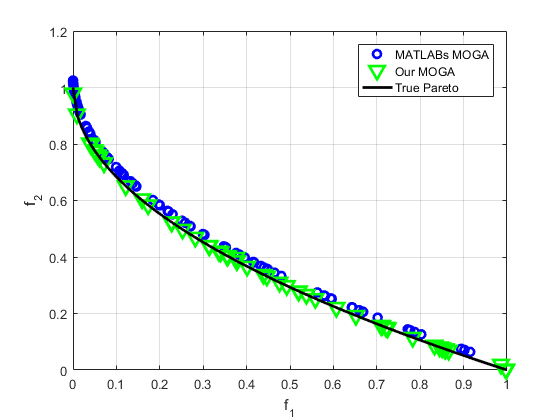
\includegraphics[width=0.85\textwidth]{ZDT1_pareto_final.png}  
  \label{fig:ZDT1}
\end{figure}

\begin{table}[h]
\caption{Quality Metrics for ZDT1} 
\centering 
\begin{tabular}{|c|c|c|} 
\hline\hline  
Metric & MATLABs MOGA & Our MOGA \\ \hline
CD & 0.3874 (0.0164) &  0.3582 (0.0040) \\ \hline
OS & 0.9605 (0.1088) & 0.9283 (0.0928) \\ \hline
\end{tabular}
\label{tab:ZDT1} 
\end{table}
\begin{figure}[h]
  \caption{ZDT1 Quality Metrics}
  \centering
  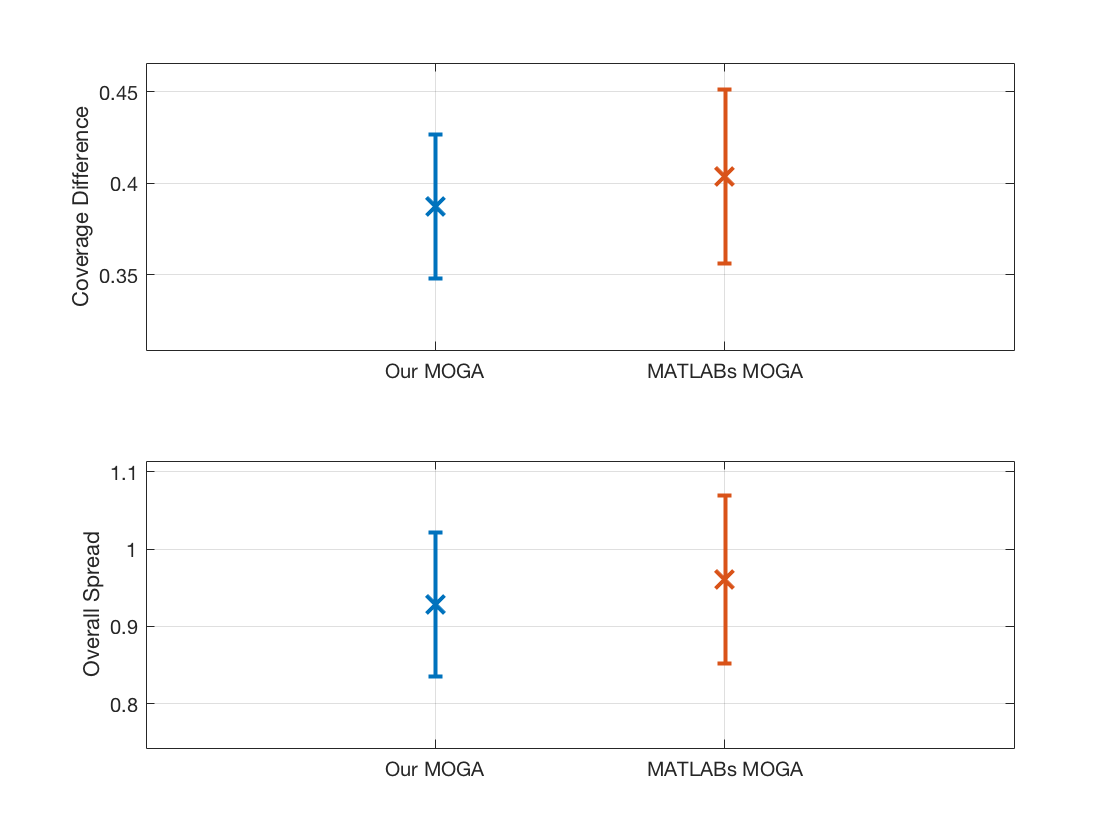
\includegraphics[width=0.85\textwidth]{ZDT1_QM.png}  
  \label{fig:ZDT1_QM}
\end{figure}

\noindent From these metrics, there is certainly a trade-off between MATLABs MOGA and the MOGA developed in this project. The coverage difference of the new MOGA is lower (and therefore superior) in this problem whereas the Pareto spread is improved when using MATLABs MOGA. 


\newpage
\subsection{ZDT2} 
The second test problem, denoted as ZDT2 in \cite{deb2001multi} is shown below. 


\begin{align*}
\textrm{Minimize} ~~~~~ f_1(\textbf{x}) &= x_1 \\
\textrm{Minimize} ~~~~~ f_2(\textbf{x}) &= g(x)*h(x) \\
\textrm{where} ~~~~~~~~~~ g(x) &= 1+\frac{9}{(n-1)}\sum_{i=2}^{n}x_i \\
~~~~~~~~~~ h(x) &= 1- \frac{f_1(x)}{g(x)}^2 \\
~~~~~~~~~~ n &= 30 \\
0 &\leq  \textbf{x}  \leq 1 \\
\end{align*}

\noindent The true Pareto frontier for this problem, similar to ZDT1, occurs when $x_i$ = 0 for i = 2,...,30. Selected parameters were similar to ZDT1 where $\alpha = 0.5$, $\sigma=0.5$, $\epsilon=0.22$; the number of chromosomes was 300. Figure~\ref{fig:ZDT2} shows a sample result from both MATLABs built in MOGA and the MOGA developed in this project. Table~\ref{tab:ZDT2} summarizes the mean quality metrics for each algorithm over ten runs.
\begin{figure}[H]
  \caption{Example Pareto Results for ZDT2}
  \centering
  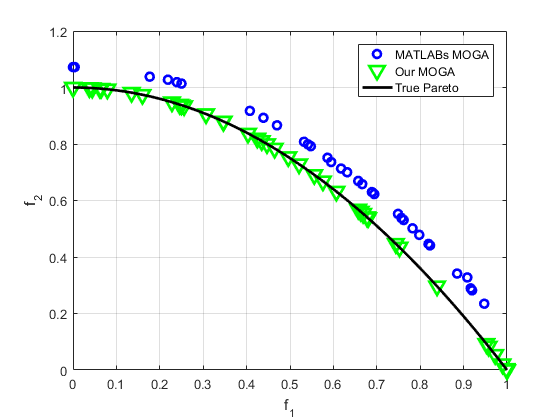
\includegraphics[width=0.85\textwidth]{ZDT2_pareto_final.png}  
  \label{fig:ZDT2}
\end{figure}

\begin{table}[H]
\caption{Quality Metrics for ZDT2} 
\centering 
\begin{tabular}{|c|c|c|} 
\hline\hline  
Metric & MATLABs MOGA & Our MOGA \\ \hline
CD & 0.7832  (0.0821) & 0.6971  (0.0094) \\ \hline
OS &  0.8781 (0.0946) & 1.0086 (0.0278)  \\ \hline
\end{tabular}
\label{tab:ZDT2} 
\end{table}
\begin{figure}[H]
  \caption{ZDT2 Quality Metrics}
  \centering
  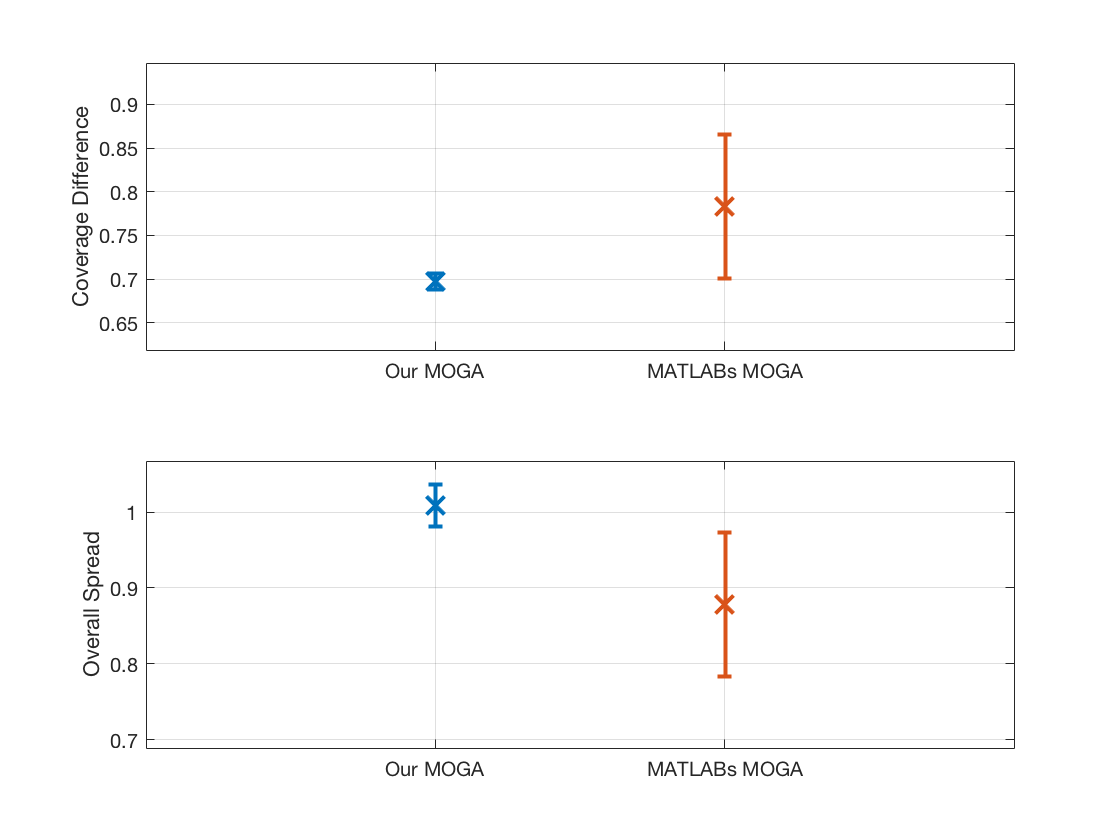
\includegraphics[width=0.85\textwidth]{ZDT2_QM.png}  
  \label{fig:ZDT2_QM}
\end{figure}
\newpage
\newpage
\newpage
\goodbreak
\newpage
    
\goodbreak

\newpage
\goodbreak
\subsection{ZDT3} 
The third test problem, denoted as ZDT3 in \cite{deb2001multi} is shown below. 


\begin{align*}
\textrm{Minimize} ~~~~~ f_1(\textbf{x}) &= x_1 \\
\textrm{Minimize} ~~~~~ f_2(\textbf{x}) &= g(x)*h(x) \\
\textrm{where} ~~~~~~~~~~ g(x) &= 1+\frac{9}{(n-1)}\sum_{i=2}^{n}x_i \\
~~~~~~~~~~ h(x) &= 1- \sqrt{\frac{f_1(x)}{g(x)}}- \frac{f_1(x)}{g(x)}\sin(10\pi f_1) \\
~~~~~~~~~~ n &= 30 \\
0 &\leq  \textbf{x}  \leq 1 \\
\end{align*}

\noindent The true Pareto frontier for this problem again occurs when $x_i$ = 0 for i = 2,...,30. The fitness parameters selected in this problem were $\alpha = 1$, $\sigma = 0158$ and $\epsilon = 0.22$. Again, the number of chromosomes in this problem was 300. Figure~\ref{fig:ZDT3} shows a sample result from both MATLABs built in MOGA and the MOGA developed in this project. Table~\ref{tab:ZDT3} summarizes the mean quality metrics for each algorithm for ten runs. \newline

\begin{figure}[H]
  \caption{Example Pareto Results for ZDT3}
  \centering
  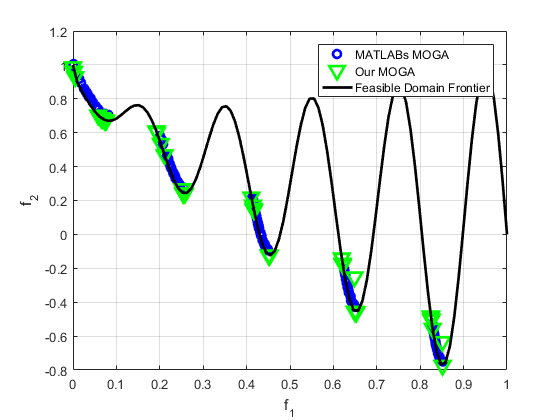
\includegraphics[width=0.85\textwidth]{ZDT3_pareto_final.png}  
  \label{fig:ZDT3}
\end{figure}

\begin{table}[H]
\caption{Quality Metrics for ZDT3} 
\centering 
\begin{tabular}{|c|c|c|} 
\hline\hline  
Metric & MATLABs MOGA & Our MOGA \\ \hline
CD & 0.7407 (0.0050) & 0.7554 (0.0031) \\ \hline
OS & 0.8565 (0.0098) & 0.8489 (0.0180) \\ \hline
\end{tabular}
\label{tab:ZDT3} 
\end{table}
\begin{figure}[h]
  \caption{ZDT3 Quality Metrics}
  \centering
  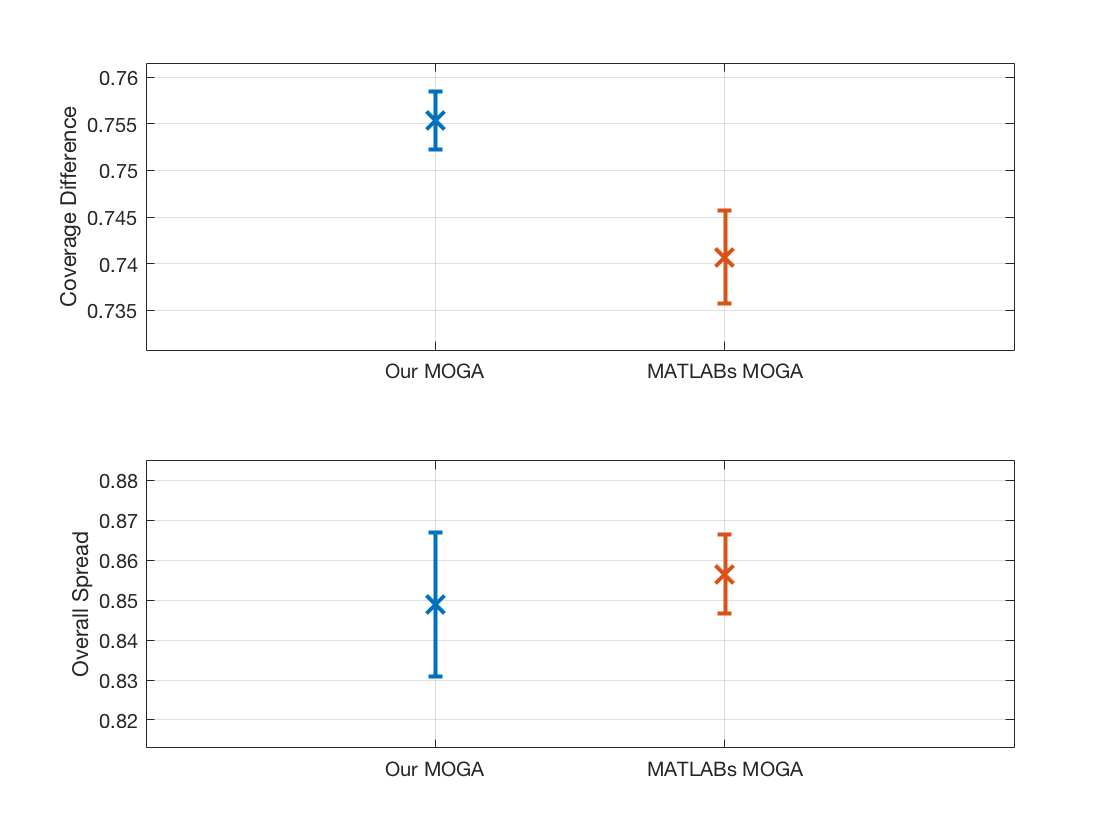
\includegraphics[width=0.85\textwidth]{ZDT3_QM.png}  
  \label{fig:ZDT3_QM}
\end{figure}

\noindent Overall, MATLABs MOGA outperforms the MOGA developed in this project in both coverage difference and Pareto spread. A paired t-test shows that the difference in the means for coverage difference is statistically significant (p<0.05), while the difference is not statistically significant in Pareto Spread (p=0.21). \newline

\section{Constrained MOGA Problems}

There are many ways in which fitness evaluation can be accomplished for constrainted problems. In general, some factors which may be included in fitness evaluation are the feasibility of an individual, the amount of infeasibility, and the number of violated constraints for a certain individual. Several methods to take into account these factors are described in \cite{kurpati2002constraint}. For this project, all three parameters are used to evaluated the fitness of individuals in constrained problems. This method is denoted at CH-I4 in \cite{kurpati2002constraint}. \newline

\noindent As in the unconstrained algorithm, there are fitness parameters which can be chosen to place more or less emphasis on any of the factors (i.e., amount of feasibility, etc.). For each test problem, these factors were chosen such that the "best" resulting Pareto frontier could be obtained. "Best", here is meant to describe the Pareto spread and coverage difference of the resulting frontier. The two factors which could be tuned in this algorithm were denoted as CF1 and CF2. CF1 is the factor affects the emphasis on the amount of infeasibility of an individual. Whereas CF2 affects the emphasis on the number of violated constraints. \newline

\noindent The following sections shall discuss the test problems OSY, TNK, and CTP, the results from the constrained fitness function with MATLAB's "ga" function and from MATLAB's "gamultiobj". 


\subsection{OSY} 
This test problem, denoted as OSY in \cite{deb2001multi} is shown below, Figure~\ref{fig:OSY_true} shows the true Pareto frontier for this problem. The factors chosen for this problem were $CF1 = 0.005$ and $CF2 = 0.015$, this placed a higher weight of the number of constraint violations than the amount of infeasibility. 


\begin{align*}
\textrm{Minimize} ~~~~~ f_1(\textbf{x}) &= -(25(x_1-2)^2+(x_2-2)^2+(x_3-1)^2+(x_4-4)^2+(x_5-1)^2) \\
\textrm{Minimize} ~~~~~ f_2(\textbf{x}) &= \sum_{i=1}^{6}x_i^2 \\
\textrm{Subject to} ~~~~ g_1(x) &= 1-\frac{x_1+x_2}{2} \leq 0 \\
g_2(x) &= \frac{x_1+x_2}{6}-1 \leq 0 \\
g_3(x) &= \frac{x_2-x_1}{2}-1 \leq 0 \\
g_4(x) &= \frac{x_1-3x_2}{2}-1 \leq 0 \\
g_5(x) &= \frac{(x_3-3)^2+x_4}{4}-1 \leq 0 \\
g_6(x) &= 1-\frac{(x_5-3)^2+x_6}{4} \leq 0 \\
0 &\leq  x_1,x_2,x_6  \leq 10 \\
1 &\leq  x_3,x_5  \leq 5 \\
0 &\leq  x_4  \leq 6 \\
\end{align*}
\begin{figure}[H]
  \caption{True Pareto Frontier for OSY}
  \centering
  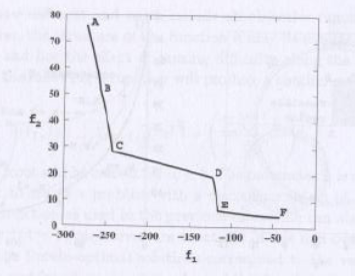
\includegraphics[width=0.85\textwidth]{OSY_pareto_true.png}  
  \label{fig:OSY_true}
\end{figure}

\noindent Figure~\ref{fig:OSY} shows a sample result from both MATLABs built in MOGA and the MOGA developed in this project. Table~\ref{tab:OSY} summarizes the mean quality metrics for each algorithm for ten runs.
\begin{figure}[h]
  \caption{Example Pareto Results for OSY}
  \centering
  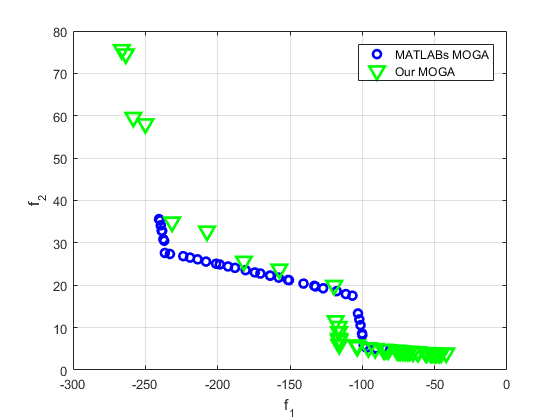
\includegraphics[width=0.85\textwidth]{OSY_pareto_final.png}  
  \label{fig:OSY}
\end{figure}

\begin{table}[H]
\caption{Quality Metrics for OSY} 
\centering 
\begin{tabular}{|c|c|c|} 
\hline\hline  
Metric & MATLABs MOGA & Our MOGA \\ \hline
CD & 0.7882 (0.1995) & 0.5507 (0.0685)  \\ \hline
OS & 0.5322 (0.3393) & 0.9608 (0.2427) \\ \hline
\end{tabular}
\label{tab:OSY} 
\end{table}
\begin{figure}[H]
  \caption{OSY Quality Metrics}
  \centering
  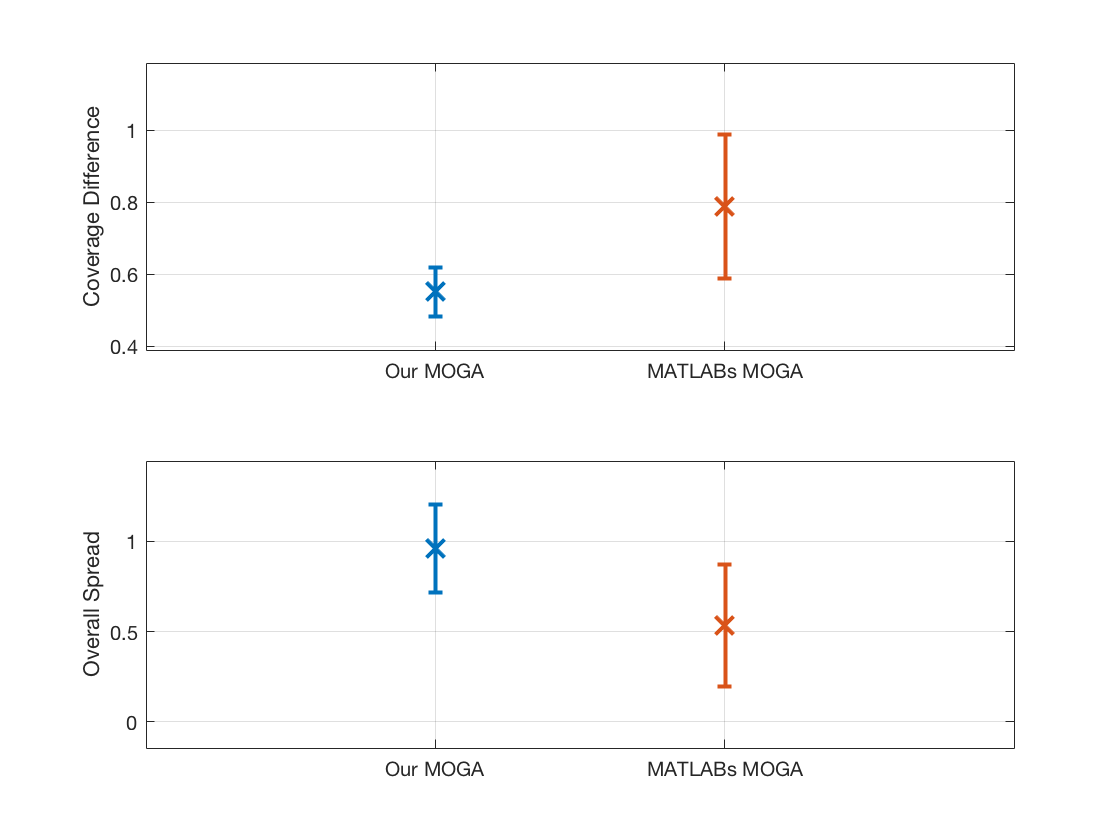
\includegraphics[width=0.85\textwidth]{OSY_QM.png}  
  \label{fig:OSY_QM}
\end{figure}
\newpage
\subsection{TNK} 
This test problem, denoted as TNK in \cite{deb2001multi} is shown below with the true Pareto frontier shown in Figure~\ref{fig:TNK_true}. Constraint parameters CF1 and CF2 were both chosen to be 0.01 to place equal emphasis on amount of infeasibility and number of violated constraints.

\begin{align*}
\textrm{Minimize} ~~~~~ f_1(\textbf{x}) &= x_1 \\
\textrm{Minimize} ~~~~~ f_2(\textbf{x}) &= x_2 \\
\textrm{Subject to} ~~~~ g_1(x) &= -x_1^2-x_2^2+1+0.1\cos(16\arctan(\frac{x_1}{x_2})) \leq 0 \\
g_2(x) &= (x_1 - 0.5)^2 + (x_2 - 0.5)^2 -0.5 \leq 0 \\
0 &\leq  x_1,x_2 \leq \pi \\
\end{align*}
\begin{figure}[H]
  \caption{True Pareto Frontier for TNK}
  \centering
  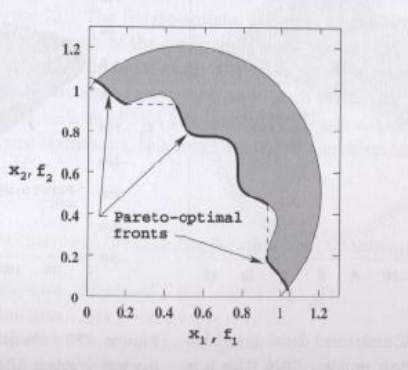
\includegraphics[width=0.85\textwidth]{TNK_pareto_true.png}  
  \label{fig:TNK_true}
\end{figure}


\noindent Figure~\ref{fig:TNK} shows a sample result from both MATLABs built in MOGA and the MOGA developed in this project. Table~\ref{tab:TNK} summarizes the mean quality metrics for each algorithm for ten runs.
\begin{figure}[h]
  \caption{Example Pareto Results for TNK}
  \centering
  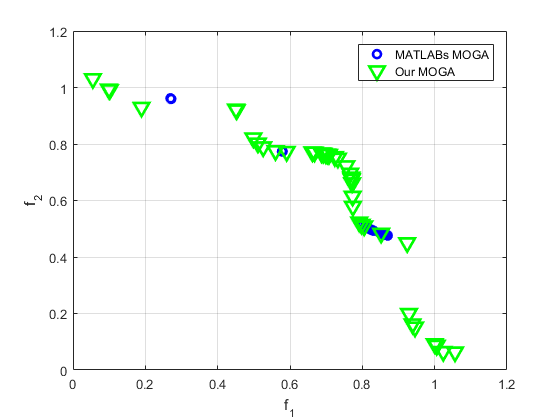
\includegraphics[width=0.85\textwidth]{TNK_pareto_final.png}  
  \label{fig:TNK}
\end{figure}

\begin{table}[H]
\caption{Quality Metrics for TNK} 
\centering 
\begin{tabular}{|c|c|c|} 
\hline\hline  
Metric & MATLABs MOGA & Our MOGA \\ \hline
CD &  0.8581 (0.0480) & 0.7792 (0.0036) \\ \hline
OS & 0.4177 (0.3216) & 0.9763 (0.0178)\\ \hline
\end{tabular}
\label{tab:TNK} 
\end{table}
\begin{figure}[H]
  \caption{TNK Quality Metrics}
  \centering
  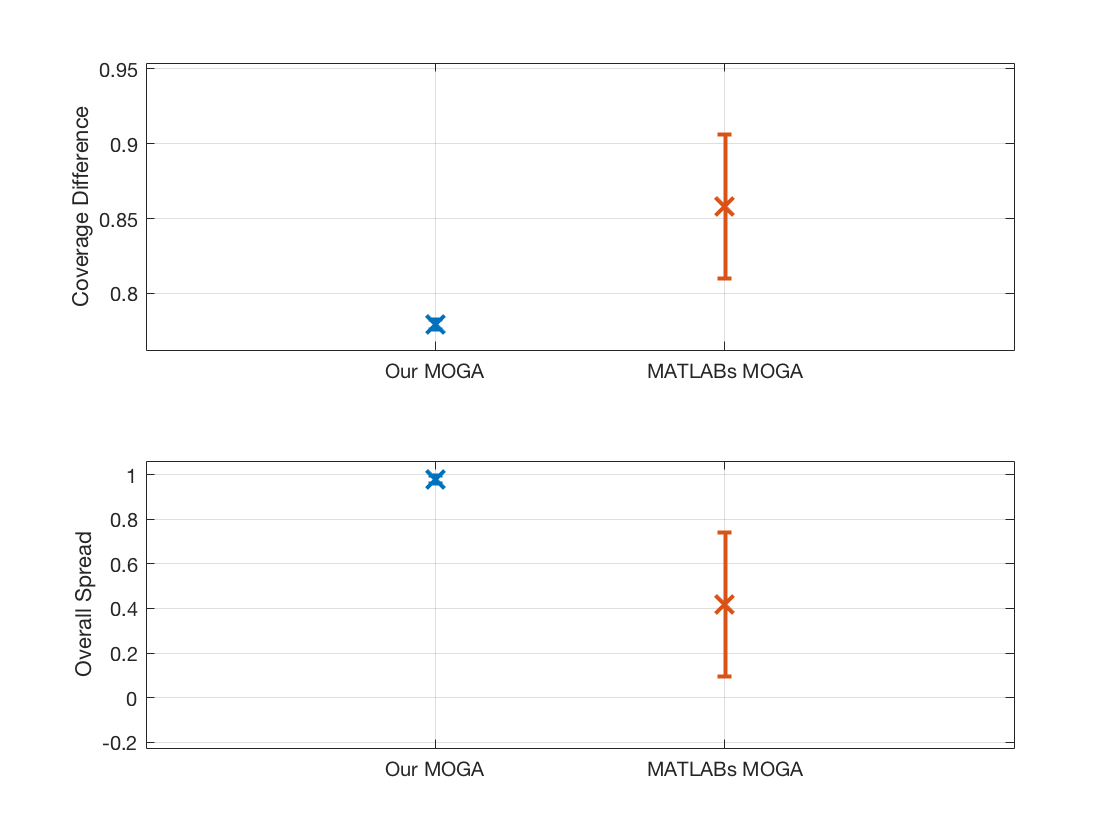
\includegraphics[width=0.85\textwidth]{TNK_QM.png}  
  \label{fig:TNK_QM}
\end{figure}
 
\noindent Comparing the estimated Pareto frontiers to the true Pareto frontier, is is clear that our MOGA outperforms MATLAB's MOGA. The Pareto spread in our MOGA is significantly higher however the coverage difference is higher in MATLABs MOGA (p<0.05).
\newpage
\subsection{CTP} 
This test problem, denoted as CTP in \cite{deb2001multi} is shown below and the true Pareto frontier is shown in Figure~\ref{fig:CTP_true}. Just as in TNK, constraint parameters CF1 and CF2 were both chosen to be 0.01 to place equal emphasis on amount of infeasibility and number of violated constraints.


\begin{align*}
\textrm{Minimize} ~~~~~ f_1(\textbf{x}) &= x_1 \\
\textrm{Minimize} ~~~~~ f_2(\textbf{x}) &= g(x)(1-\sqrt{\frac{f_1(x)}{g(x)}} \\
\textrm{Subject to} ~~~~ g_1(x) &= a|\sin(b\pi(\sin(\theta)(f_2(x)-e)+\cos(\theta)f_1(x))^c)|^d \\
&- \cos(\theta)(f_2(x)-e)-\sin(\theta)f_1(x) \leq 0 \\
\textrm{where} ~~~~~~~~~~ \theta &= -0.2\pi, a = 0.2, b=10, c=1, d=6, e = 1 \\
g(x) &= |1+(\sum_{i=2}^{10}x_i)^{0.25}| \\
0 &\leq  x_1  \leq 1 \\
-5 &\leq  x_i  \leq 5, i = 2,...,10 \\
\end{align*}
\begin{figure}[H]
  \caption{True Pareto Frontier for CTP}
  \centering
  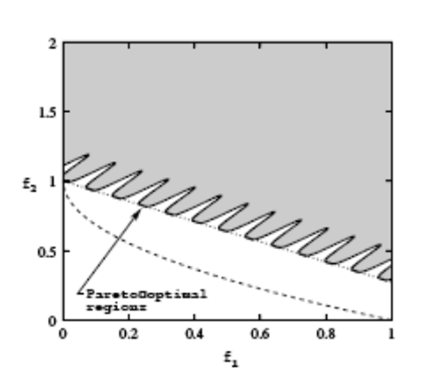
\includegraphics[width=0.85\textwidth]{CTP_pareto_true.png}  
  \label{fig:CTP_true}
\end{figure}

\noindent Figure~\ref{fig:CTP} shows a sample result from both MATLABs built in MOGA and the MOGA developed in this project. Table~\ref{tab:CTP} summarizes the mean quality metrics for each algorithm for ten runs \cite{deb2001multi}.
\begin{figure}[h]
  \caption{Example Pareto Results for CTP}
  \centering
  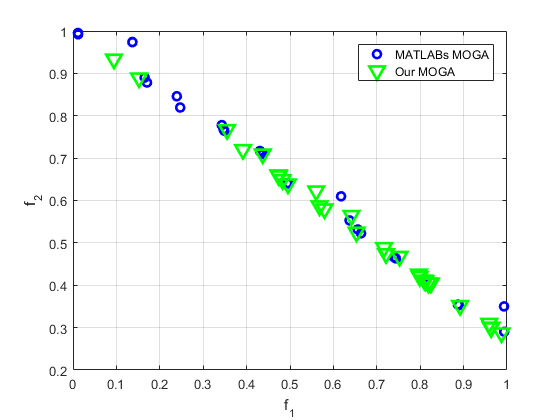
\includegraphics[width=0.85\textwidth]{CTP_pareto_final.png}  
  \label{fig:CTP}
\end{figure}

\begin{table}[H]
\caption{Quality Metrics for CTP} 
\centering 
\begin{tabular}{|c|c|c|} 
\hline\hline  
Metric & MATLABs MOGA & Our MOGA \\ \hline
CD & 0.6802 (0.0067) &  0.6802 (0.0092) \\ \hline
OS & 0.7901 (0.0734) & 0.5959 (0.1324) \\ \hline
\end{tabular}
\label{tab:CTP} 
\end{table} 
\begin{figure}[H]
  \caption{CTP Quality Metrics}
  \centering
  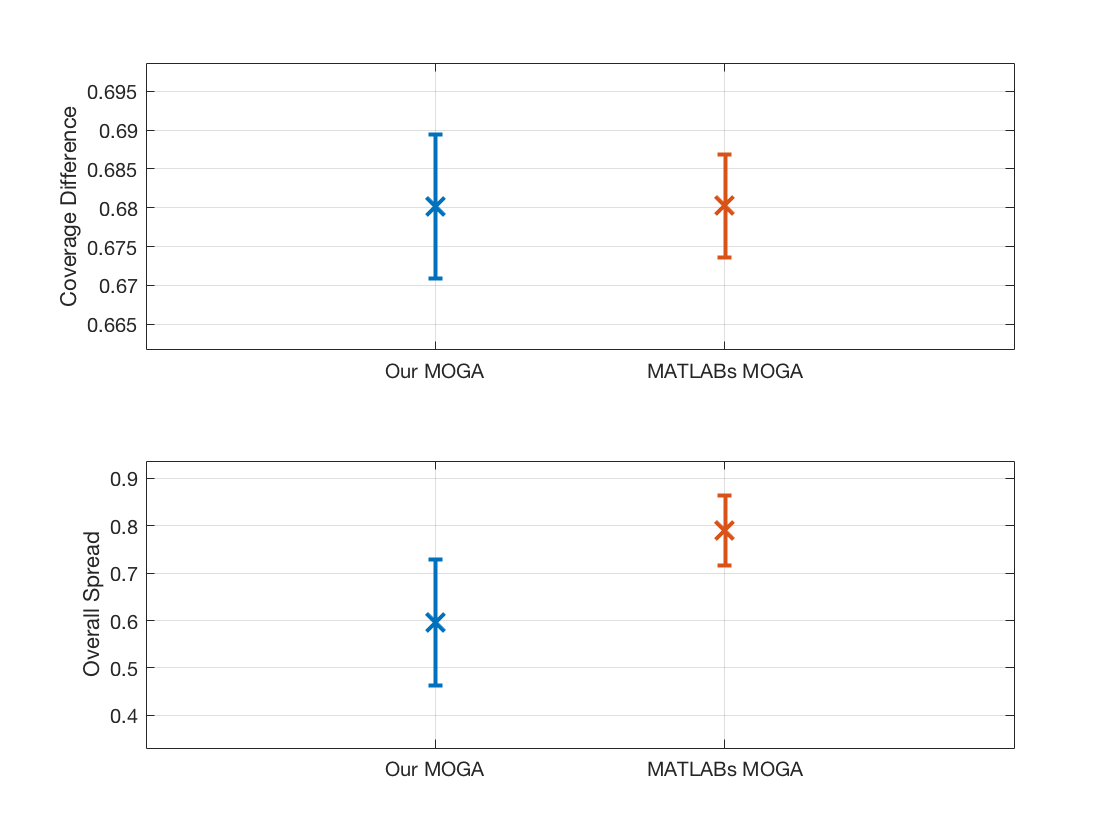
\includegraphics[width=0.85\textwidth]{CTP_QM.png}  
  \label{fig:CTP_QM}
\end{figure}
 
\noindent The mean values for coverage difference are exactly the same for both algorithms. In fact a paired t-test also shows the means are not statistically difference(p>0.05). For Pareto spread, MATLAB's MOGA performs the highest.
\newpage
\section{Robust Problems} 
To solve problems with an uncertain variable we implement RMOGA.  One way to ensure robustness for a given population considered in GA, is by finding the value of the uncertain variable which maximizes the constraint values acording to each member in the population.  Another way is to discretize the dependent variable and then find which uncertain variable in this set maximizes the constraint values.  This latter method is the one we chose because of the decreased execution time over the former.  These two options are shown in figure \ref{fig:discretize}.
   Since the uncertainty term only appears in the constraints portion of both of the problems we consider this discretization is fairly simple.  In addition, since the uncertain terms are linearly combined in the constraints, this discretization is trivial.


\begin{figure}[H]
  \caption{Options for making optimization robust to uncertain variables. }
  \centering
  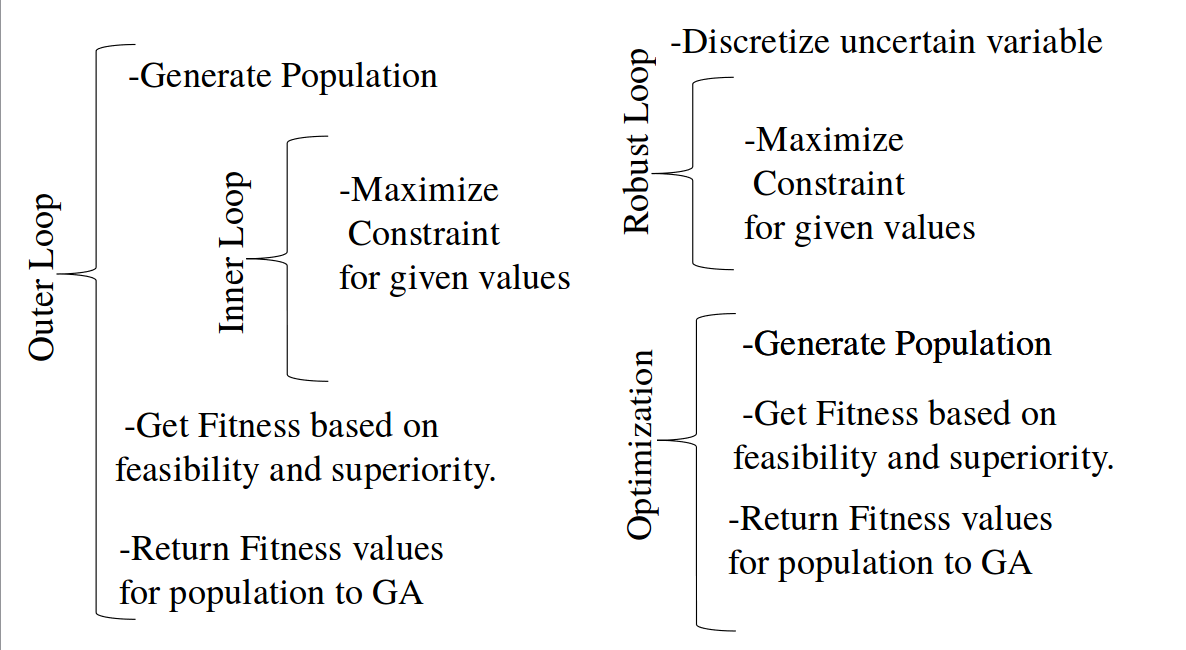
\includegraphics[width=0.85\textwidth]{Robustness.png}  
  \label{fig:discretize}
\end{figure}


 
\subsection{Robust TNK} 
This test problem, denoted as TNK in \cite{deb2001multi} is shown below with the true Pareto frontier shown in Figure~\ref{fig:TNK_true}.

\begin{align*}
\textrm{Minimize} ~~~~~ f_1(\textbf{x}) &= x_1 \\
\textrm{Minimize} ~~~~~ f_2(\textbf{x}) &= x_2 \\
\textrm{Subject to} ~~~~ g_1(x) &= 1+0.1\cos(16\arctan(\frac{x_1}{x_2})) + \\
&~~~~ 0.2\sin{p_1}\cos{p_2} -x_1^2-x_2^2\leq 0 \\
g_2(x) &= (x_1 - 0.5)^2 + (x_2 - 0.5)^2 -0.5 \leq 0 \\
0 &\leq  x_1,x_2 \leq \pi \\
-1& \leq p \leq 3\\
\end{align*}

\noindent Figure~\ref{fig:robust} shows a sample result from both MATLABs built in MOGA and the robust MOGA developed in this project. Table~\ref{tab:robustTNK} summarizes the mean quality metrics for each algorithm for ten runs. \newline
\begin{figure}[H]
  \caption{Example Pareto Results for TNK}
  \centering
  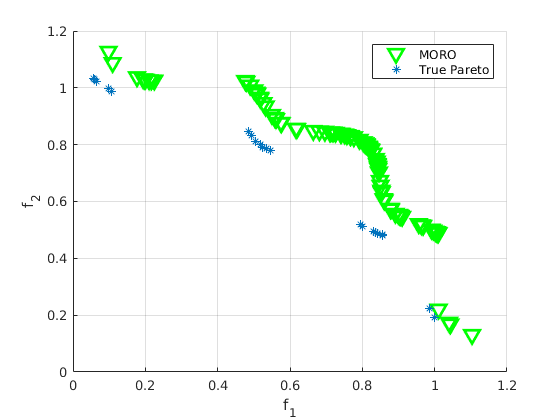
\includegraphics[width=0.85\textwidth]{prob7_nChr25_nRun400.png}  
  \label{fig:robustTNK}
\end{figure}

\begin{table}[H]
\caption{Quality Metrics for Robust TNK (10 Runs)} 
\centering 
\begin{tabular}{|c|c|c|} 
\hline\hline  
Metric &  Our MOGA \\ \hline
CD & 0.95 (0.014) \\ \hline
OS & 0.66 (0.012) \\ \hline
\end{tabular}
\label{tab:robustTNK} 
\end{table}
 
\noindent Comparing the estimated Pareto frontiers to the true Pareto frontier, is is clear that our MOGA outperforms MATLAB's MOGA. The Pareto spread in our MOGA is significantly higher however the coverage difference is higher in MATLABs MOGA (p<0.05).
 
\subsection{Flight Planning Problem (FPP)}
Now let us consider the final problem where we try to minimize the total flight time from the start location $(0,12.5)$ to the finish location $(40,12.5)$.  In this problem there is a know wind velocity field which changes the total velocity of the aircraft with respect to the ground.  At the same time, we want to maximize the distance of the flight path from some group of some exclusion zones. This also introduces a constraint that requires the flight path not intersect the exclusion zone. Each exclusion zone is approximated by a circle with known centers.  The radius of each exclusion zone is known to $\pm 2m$.  As a result this problem can be approached as a bi-objective optimization with a robust feasibility constraint. 

\begin{align*}
\textrm{Minimize} ~~~~~ f_1(\textbf{x},\textbf{y}) &= flightTime(\textbf{x},\textbf{y})\\
\textrm{Maximize} ~~~~~ f_2(\textbf{x},\textbf{y}) &= -\min_{i,j}\sqrt{(\textbf{x}_i-\textbf{xc}_j)^2 + (\textbf{y}_i-\textbf{yc}_j)^2}\\
\textrm{Subject to} ~~~~ \textbf{g}_j(\textbf{x},\textbf{y}) &= -\min_{j}\left[\textbf{r}_j+p_0 + \Delta p -\sqrt{(\textbf{x}_i-\textbf{xc}_j)^2 + (\textbf{y}_i-\textbf{yc}_j)^2}\right]   \leq 0 \\
\textrm{where} ~~~~~~~~~~ 
0 &\leq  x \leq 50, i = 2,...,10 \\
0 &\leq  y  \leq 25, i = 2,...,10 \\
&p_0 = 0\\
&\Delta p \in [0,2] \\
\end{align*}

\noindent The function $flightTime(\textbf{x},\textbf{y})$ is a black-box. The values $\textbf{xc}_j$ and  $\textbf{yc}_j$ specify the exclusion zone centers while $\textbf{r}_j$ specify the radii. A solution to this problem is shown in figure \ref{fig:FPP}.  In this figure there are two exclusion zones.
\begin{figure}[H]
  \caption{True Pareto Frontier for CTP}
  \centering
  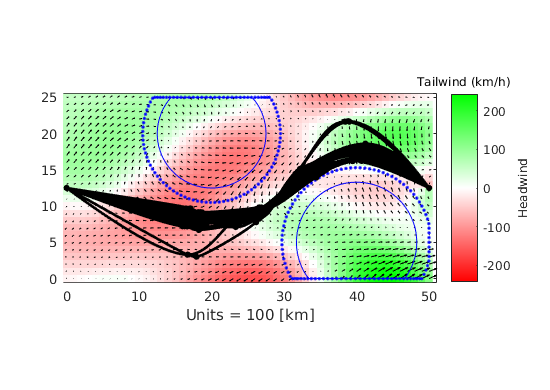
\includegraphics[width=0.85\textwidth]{FPP.png}  
  \label{fig:FPP}
\end{figure}
	
\begin{figure}[H]
  \caption{True Pareto Frontier for CTP}
  \centering
  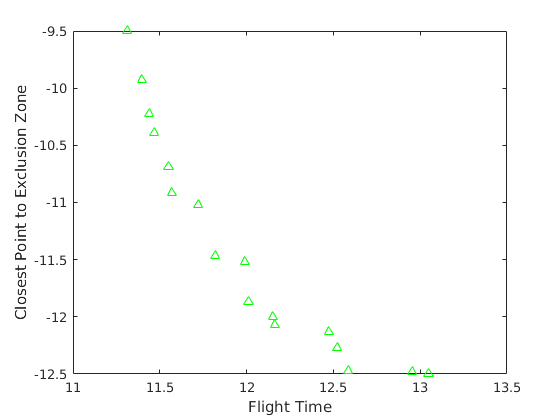
\includegraphics[width=0.85\textwidth]{FPP_pareto.png}  
  \label{fig:FPP_pareto}
\end{figure}

\begin{table}[H]
\caption{Quality Metrics for Robust FPP (10 Runs)} 
\centering 
\begin{tabular}{|c|c|c|} 
\hline\hline  
Metric &  Our MOGA \\ \hline
CD & 0.2427 (0.0704) \\ \hline
OS & 0.4794 (0.1220) \\ \hline
\end{tabular}
\label{tab:robustTNK} 
\end{table}




%
%\begin{table}[h]
%\caption{Quality Metrics for Robust FPP with waypoint constraints(10 Runs)} 
%\centering 
%\begin{tabular}{|c|c|c|} 
%\hline\hline  
%Metric &  Our MOGA \\ \hline
%CD & 0.27 0.0269) \\ \hline
%OS & 0.4794 (0.1220) \\ \hline
%\end{tabular}
%\label{tab:robustTNK} 
%\end{table}

\section{Conclusion}

Overall, it was found that different optimization algorithms result in a range of solutions for a given test problem. Thus it is important, when developing an optimization algorithm, to test against a range of optimization problems. In addition, it was also concluded that special attention should be paid to tunable parameters within each algorithm. Understanding the nature of the parameter and how it affects the algorithm is crucial to obtaining the "true" Pareto frontier. 


 
\vspace{-0.1in}
\bibliographystyle{IEEEtran}
\bibliography{references.bib}
 
 
\end{document}
